\documentclass[aps,prl,twocolumn,showpacs,superscriptaddress,groupedaddress,10pt]{revtex4-1}  % for review and submission
%\documentclass[aps,twocolumn,floatfix,prl,10pt]{revtex4-1}
%\documentclass[letterpaper,10pt,prl,twocolumn,aps]{revtex4-1}
%\documentclass[aps,preprint,floatfix,prl]{revtex4-1}
%\usepackage{fullpage}
\usepackage{amsmath}
\usepackage{amsfonts}
\usepackage{amssymb}
\usepackage{graphicx}
%\usepackage{slashbox}
\usepackage{color}
\usepackage{longtable}
\usepackage{array}
\usepackage{dashrule}
\usepackage{dcolumn}% Align table columns on decimal point
%\usepackage{dcolumn}% Align table columns on decimal point
\usepackage{bm}% bold math
\usepackage{ifthen}
\usepackage{amsthm} % Theorem Formatting
\usepackage{amssymb}	% Math symbols such as \mathbb
\usepackage{calrsfs}
\usepackage{subfigure}
\graphicspath{ {images/} }
\newcommand{\ellcap}{{\ell_\text{c}}}
\newcommand{\Fh}{{\boldsymbol{F}_h}}
\newcommand{\Fv}{{\boldsymbol{F}_v}}
\newcommand{\Tv}{{\boldsymbol{T}}}
\newcommand{\bn}{{\boldsymbol{n}}}
\newcommand{\bt}{{\boldsymbol{t}}}
\newcommand{\bz}{{\boldsymbol{z}}}
\newcommand{\bx}{{\boldsymbol{x}}}
\newcommand{\by}{{\boldsymbol{y}}}
\newcommand{\bT}{{\boldsymbol{T}}}
\newcommand{\bu}{\mathbf{u}}
\newcommand{\grad}{\mathbf{\nabla}}
\newcommand{\del}{\partial}


\begin{document}
\title{Waving and swaying}
\author{Ravi Singh, Shreyas Mandre}
\affiliation{Brown University, Providence RI 02912 USA}
\author{L. Mahadevan}
\affiliation{Harvard University, Cambridge MA 02138 USA}
\author{Mahesh Bandi\footnote{work performed while visiting Brown University}}
\affiliation{Okinawa Institute of Science and Technology, Okinawa, Japan}
\author{Amala Mahadevan}
\affiliation{Woods Hold Institute of Oceanography, Woods Hole MA USA}
%\author{Shreyas Mandre}
%\affiliation{Brown University, Providence RI 02912 USA}

\begin{abstract}
%The spontaneous waving of marine grass is thought to be due to a Kelvin-Helmholtz instability resulting from an inflection point in the flow profile. 
%We find that this inflection point is located inside the grass canopy but it does not lead to Kelvin Helmholtz instability which is 
%normally observed in a free shear layer. We also show that the wavelength of coherent vortices scales with the unvegetated water depth, and not with 
%the shear layer thickness as predicted by a theory based on Kelvin-Helmholtz instability. Based on these results, we propose a mechanism for waving 
%marine grass based on the shear instability of the flow above the canopy.

%The spontaneous waving of marine grass is though to be due to a Kelving-helmholtz instability resulting from strong shear near top of grass. On the contrary
%we find that strong velocity shear resulting from vertical discontinuity of drag due to presence of grass does not lead to Kelvin-Helmholtz instability which is 
%normally observed in free shear flows. We also show that wavelength of coherent vortices scales with the unvegetated water depth. Based on these results, 
%we propose an alternative mechanism which attributes waving of marine grass on shear instability of flow above the canopy. 

The spontaneous waving of marine grass is thought to be due to a Kelvin-Helmholtz instability resulting from an inflection point in the flow profile. We find that this inflection point
is located near the tip of grass canopy. Our analysis shows that flow in presence of grass become unstable not only through a mechanism of Kelvin-Helmholtz instability associated with 
inflection point but also through shear instability of flow above grass coupled with the porous flow through grass bed.
\end{abstract}
\maketitle

\section{Introduction}
Sea grasses exhibit rich set of dynamics due to their interaction with the flow of water and can considerably affect surrounding hydrodynamic conditions.
Resulting changes in hydrodynamic conditions can influence number of environmental variables and processes such as 
transport of sediments, contaminants, dissolved oxygen, plant growth and biomass production etc \cite{Fonseca87}\cite{Nepf99}. 
The response of flexible grass canopies to steady current in form of large amplitude coherent oscillation, known as mo-nami \cite{AckermanOkubo93}, plays a central role
in the recruitment of microscopic marine organism such as blue mussel larvae \cite{Grizzle96}. The hydrodynamic mechanism underlying monami is the focus of this paper. 
\newline
Similar phenomenon of large amplitude coherent oscillation of canopy in atmospheric flow known as ho-nami\cite{Inoue56}\cite{Raupach96}, have also been observed.
A crucial difference between the atmospheric and aquatic flow is that the atmospheric flows are essentially unbounded vertically. Another major
difference between the two is the considerable difference of stiffness of canopies; terrestrial canopies tend to be much more rigid than aquatic canopies.
Due to these differences between aquatic and marine flow, our analysis of flow in presence of flexible grass in a bounded domian is applicable only to marine canopies. 
\newline   
Existing explanation of mo-nami invokes the existence of strong shear near the top of the canopy \cite{Ghisal02}\cite{Raupach96} (Ghisalberti 2002, Raupach 1996) due to
different amounts of drag experienced by fluid in and above the canopy. This shear layer is assumed to become unstable to coherent vortices through a mechanism similar to 
Kelvin-Helmholtz instability. Influence of these coherent eddies over sea grasses is manifested in their large amplitude synchronous oscillations.
%Sea grasses exhibit large amplitude wave like motion in response to these eddies propagating downstream.
%are exhibited in form of large amplitude oscillations knows as mo-nami.
\newline
While shear layer model successfully predict frequency of mo-nami for number of experimental observations,
several aspect of existing theory remain unexplained. First, linear stability analysis of base flow does not take into account influence of drag due to grass hence not a self 
consistent theory. Second, classical free shear flow is known to be unstable above a very small Reynolds number $\leq 10 $, whereas observed critical 
Reynolds number\cite{Grizzle96} (Grizzle 1996) for monami is much higher $\approx O(1000)$. These drawbacks of existing theory suggest that flow through vegetation requires 
further investigation for better understanding of phenomenon.
\newline 
In this paper we extend the idea of Raupach et.al\cite{Raupach96} via incorporating drag due to presence of vegetation. Our calculation of linear stability analysis of flow in presence of grass
shows that flow through vegetation become unstable not only through a mechanism of Kelvin-Helmholtz 
instability associated with strong shear near the canopy top but also through shear instability of flow above grass canopies and shear instability of flow comprising flow above the canopy 
and flow in the shear layer. We further show that inclusion of drag due to grass predicts a threshold condition for waving. We confirm our analysis by comparing prediction from theory 
with field and experimental observations.
%\section{The model}
%Monami is believed to be response to strong oscillations of flow in streamwise velocity associated with coherent vortices.
\newline  
The drag force experienced by flow due to presence of grass is believed to play a central role in the development of coherent eddies. This drag force experienced by flow depends 
primarily on flow velocity, fluid density and mean frontal area of the grass canopy. The mechanism leading to coherent eddies is believed to depend weakly on flexibility of grass
unless frequency of passage of coherent eddies is close to the natural frequency of the grass blade (Py el al 2008). Since natural frequency of a typical marine grass blades are
very small compared to the frequency of the passage of eddies observed in marine grass, we do not expect the mechanism leading to instability of flow to be affected by plant flexibility.
Therefore we replace the flexible grass with stiff structure to investigate dynamics leading to generation of coherent vortices. We use a mean field model for the coupling between the 
flow and the canopy. Drag force exerted by the grass is approximated via a 
continuous body force $\mathbf{f}=-N_g\mathbf{f_d}$ in the fluid momentum balance as
\begin{equation}
\rho \left(\bu_{t}+\bu.\grad\bu \right) = -\grad P+\mu\grad^{2}\bu +\mathbf{f}+\rho\mathbf{g}
\label{navier-stokes}
\end{equation}
%\begin{equation}
% \mathbf{f}=-N\mathbf{f_{d}}
%\end{equation}
where $\mathbf{f_{d}}$ is drag force per unit length of the grass blade, $N_g$ the grass number density per unit area, $\rho$ the fluid density, $\mathbf{u}$ the velocity, 
$P$ the pressure, $\mu$ the viscosity and $\mathbf{g}$ the acceleration due to gravity. Drag force itself is modeled 
as $\mathbf{f_{d}}=C_N \rho u_{N}^{2}d\hat{n}+C_{T}\rho u_{T}^{2}d\hat{t}$ where $d$ is average width of grass blade
$C_{N}$ and $C_{T}$ are normal and tangential drag coefficients respectively which are set to zero outside the grass; $\bu_{T}$, $\bu_{N}$ are velocity vector along and
normal to grass while $\hat{t},\hat{n}$ being unit vector along and normal to grass. We expect $C_T \ll C_N$ and take $C_T=0$ for rest of analysis. In the field such as marine
both $C_N \& N_g$ vary with distance from the bottom but we do not expect these variation to be central to the mechanism and therefore take $C_N \& N_g$ to be constants.
%\begin{equation}
% \mathbf{f_{d}}=C_N \rho\bu_{N}^{2}d\hat{n}+C_{T}\rho\bu_{T}^{2}d\hat{t}
%\end{equation}\
%\begin{equation}
%\begin{split}
% \frac{\del}{\del s}\left(T\hat{t}+N\hat{n}\right) & +\mathbf{f_{d}}+\mathbf{f_{buoy}} = 0\\
% \frac{\del M}{\del s}&-N = 0\\
% M &= B\kappa
%\end{split}
%\end{equation}
%where $C_{N}$ and $C_{T}$ are normal and tangential drag coefficients respectively; $\bu_{T}$, $\bu_{N}$ are velocity vector along and normal to grass.
%\section{Stability Analysis}
\newline
The steady uniform flow resulting from solution of \eqref{navier-stokes} is expected to be unstable, leading to coherent eddies underlying monami. Steady state flow driven by   
%We perform linear stability analysis of a base state associated with the vegetated flow to gain insight about instability characteristics of flow in presence of grass.
constant pressure gradient satisfies
$-\frac{dP}{dx}+\mu\frac{d^2U}{dy^2}+\rho C_N d N_gU^2=0$ with no slip at bottom and zero shear at top of surface. A sample solution is shown in figure (1) and 
compared with mean flow observed in lab scale experiment. Flow consist of a region of approximately constant velocity
\small$U_g \sim \sqrt{\frac{dP/dx}{\rho C_N dN_g}}$\normalsize arising from balance of drag force with pressure gradient with-in grass and a parabolic velocity 
profile in unvegetated region due to balance of viscous force and pressure gradient. No slip condition at bottom and continuity of shear stress at canopy top 
give rise to two boundary layer in the flow profile one near bottom and other near the tip of the grass. The boundary layer near the canopy top is identified 
as a free shear layer in the previous explanation of monami and its dependence on the grass density $N_g$ gives us a direct control of its thickness. 
In our model thickness of shear layer near top of grass is obtained by balance of viscous force 
with drag along with matching shear at grass tip exerted by flow in unvegetated region, which leads to shear layer 
width \small $\delta \sim  H\left(\frac{\rho U_0 H}{\mu} C_N d N_g H\right)^{-1/3}$\normalsize where \small$U_0 = \frac{dP/dxH^2}{\mu}$\normalsize is scale for velocity and
$H$ is half channel width.
\begin{figure}[htb]
  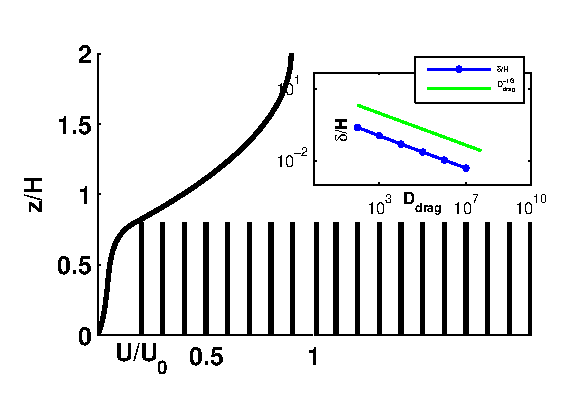
\includegraphics[scale=0.8]{fig1}
\caption{Basic flow profile (left )and model of canopy (bottom) along with variation of shear layer (inset) }
\end{figure}
\newline
Knowing the scale of shear layer we can systematically investigate its effect on flow instability
by varying grass number density $N_g$ and pressure gradient $\frac{dP}{dx}$. Considering small perturbations $u, v, p$ about the base profile $U$ and $P$
respectively, momentum and mass balance equation expanded in first order of perturbed variable yields.
\small
\begin{equation}
\begin{split}
\frac{\del u}{\del t}+U\frac{\del u}{\del x}+v\frac{\del U}{\del y} &= -\frac{1}{\rho}\frac{\del p}{\del x}+\frac{\mu}{\rho}\nabla^2u-2C_{N}dN_{g}Uu\\
\frac{\del v}{\del  t}+ U\frac{\del v}{\del x} &= -\frac{1}{\rho}\frac{\del p}{\del y}+\frac{\mu}{\rho}\nabla^2v, \hspace{0.3cm} \nabla\cdot\bu=0\\
 %\nabla\cdot \bu &= 0
\end{split}
\end{equation}
\normalsize
Momentum and mass balance equation can be non-dimensionlize using half channel height $H$, associated advection time H/$U_0$ and velocity $U_0$.
With these scaling along with the use of stream function $\psi$ with $u = \psi_{y}, v= -\psi_x$ to satisfy mass balance; momentum and mass balance can be combined 
into a single equation.
\small
\begin{equation}
R\left[\del_t+\del_x U \right]\grad^2\psi - U_{yy}\psi_x = \grad^4\psi-\frac{\del}{\del_y}\left(\frac{2}{R}\frac{H^3}{\delta^3}U\psi_y\right)
\end{equation}
\normalsize
%In most of recent work on honami/monami base profile have been approximated to a plane mixing layer profile having inflection point near top of canopy, It is also argued that 
%It is instability associated with inflection of mean velocity which is responsible for coherent eddies traveling on top of canopies. In our calculation we get base velocity
%profile by hydrodynamic balance between pressure, drag and diffusive force which also results in a velocity profile with inflection point near top of canopy with additional property 
%of having been produced through equation of motion itself.\newline
%We performed stability analysis on two different kind of base flow namely (1) flow driven by constant pressure gradient between two parallel plate (2) constant pressure gradient driven 
%flow with zero shear at top. We use following scaling to non-dimensionlize equation of motion
%Using half channel height $H$ of and associated advection time H/$U_{0}$, we use following scaling to non-dimensinlize equation 
%of motion
%   \[ u = U_{0}\bar{u},\hspace{1cm} y = (H/2)\bar{y}, \hspace{1cm} \text{with}\hspace{2mm} U_{0}=\frac{(dP/dx)H^2}{4\mu} \]
where $R= \frac{\rho U_0 H}{\mu}$ is Reynolds number. Seeking wave solution in form of $\left(u,v,\psi \right)= \left(\hat u, \hat v, \hat\phi \right)e^{ikx+\sigma t}$, 
we get generalized Orr-Sommerfield equation 
which is an eigenvalue problem. The eigenvalue $\sigma$ for a given $k$ provides growth rate and frequency associated with a perturbation of wavelength $2\pi/k$.
\small
\begin{equation}
\begin{split}
\left(\sigma+ikU\right) \left(D^2-k^2\right)\phi &= \frac{1}{R_{e}}\left[D^2 -k^{2} \right]^2\phi +ikU_{yy}\phi \\
&-\frac{\del}{\del y}\left(\frac{2}{R_e}\frac{H^3}{\delta^3}U\phi_y\right)
\label{Orr-somerfield}
\end{split}
\end{equation}
\normalsize
\begin{figure}[htb]
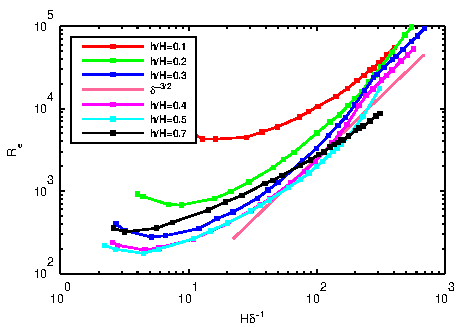
\includegraphics[]{Critical_Re_vs_delta}
\caption{Critical Reynolds number with flow for different grass height as a function of inverse shear thickness}
\label{Re_vs_delta}
\end{figure}
Solution of generalized Orr-Somerfield equation predicts a critical Reynolds number as function of grass number density, below which the flow is stable 
(Figure\ref{Re_vs_delta}). The solution also predicts a critical wavenumber $k$ with maximum growth rate.
The variation of critical wave number with the variation in $\delta$ for different grass height is shown in Figure \ref{K_vs_shear}, where we can observe that above a 
certain threshold $\delta$ the critical wavelength decreases with the decrease in $\delta$, similar to the one predicted by K-H theory based on the instability of free shear flow, for that
reason this region is identified as shear layer region. We also observe that once the $\delta$ is decreased below the threshold value, there isn't any variation in the 
critical wavelength with the decrease of shear layer thickness and $\lambda_{critical} \sim (H-h_{grass})$, we identify this region as shear instability of unvegetated region.
The boundary of transition from instability of shear-layer near the tip of grass to the instability of unvegetated flow depends on the submergence ratio of grass. 
%    This variation of critical 
%wavenumber with shear layer thickness can be divided into three distinct region. First, the region where critical wavelength does not increases linearly with the
%increase of the shear layer thickness, this region occur for canopies with thick shear layer $H/\delta <10$. Second region identified as shear layer region, where variation in critical
%wavelength is proportional to the variation in shear layer thickness, the instability in this region can be understood to arise from a mechanism similar to Kelin-Helmholtz instability 
%observed in the free shear flow. Third, the region where critical wavelength does not vary with the variation of shear layer thickness. The boundary of these region depends on 
%submergence ratio and the shear layer thickness experienced by the canopy.
\begin{figure}[htb]
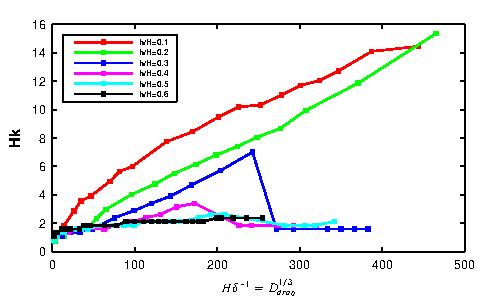
\includegraphics[]{K_vs_shear_width_noshear}
\caption{Critical Wavenumber for different grass height as function of shear layer thickness}
\label{K_vs_shear}
\end{figure}
\begin{figure}[htb]
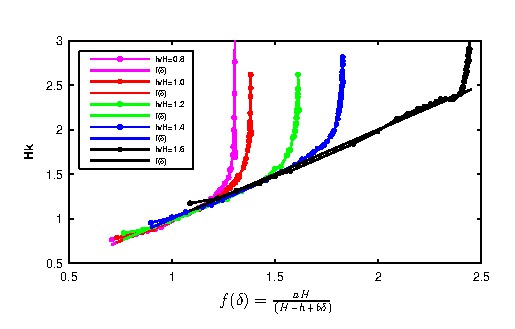
\includegraphics[]{Low_drag_k}
\caption{Critical Wavenumber for different grass height as function of $f(\delta)$}
\label{Low_drag_k}
\end{figure}
\newline
The mechanism similar to Kelvin-Helmholtz instability is observed for a wide range of shear layer thickness $5 <H/\delta <800$ for canopy with low submergence ratio $h/H\leq 0.4$.
Canopy with low submergence ratio can also be related to the canopy in unbounded flow, such as terrestrial canopy with atmospheric flow with $h/H\sim 0$. 
The linear variation of critical wavelength with the shear layer thickness in this regime is also consistent with the observed wavelength of honami for terrestrial canopies.
However, the deviation of critical wavelength from the prediction based on the instability of shear layer in region-1 and region-3 for a given submergence ratio shows the existence of 
regimes where flow instability does not arise from mechanism similar to Kelvin-Helmholtz instability. The instability in region-1 is understood to be arising from instability of flow
comprising flow in shear layer and flow above the canopies. The instability of flow comprising flow in shear layer and flow above the vegetation can be endorse by the linear 
variation of the critical wavelength with the $H-h+b\delta$ in Figure \ref{Low_drag_k}, where $b\delta$ is the amount of perturbation of the flow into the vegetation.
\newline
The constant value of critical wavelength for all the shear layer smaller than a critical value in region-3 suggest that the instability 
in the region-3 is arising from the shear instability of flow above the canopy. The existence of a regime dominated by shear instability of flow above grass is further corroborated 
by the collapse of eigen-modes for different $\delta<\delta_{cr}$ ($\delta/H=0.0037,0.0034,0.0024$ in Figure\ref{Asymptotic_mode}) into a single profile as shown in 
Figure \ref{Asymptotic_mode}, where $\delta_{cr}$ is the critical shear layer thickness
below which instability of vegetated flow arise through the mechanism of shear instability of flow in unvegetated region rather than through the mechanism of Kelvin-Helmholtz type 
instability of shear layer ($\delta/H=0.0052,0.0042$ in Figure \ref{Asymptotic_mode}). The regime of shear instability of flow above the 
grass further predicts that for large drag $R_e \sim (\frac{\delta}{H})^{-3/2}$, which can be understood by asymptotic analysis of \eqref{Orr-somerfield}.
Noting that for large drag, non-dimensional flow velocity $U \sim (\frac{\delta}{H})^{3/2}$ inside the grass and $R_{e} \gg 1$. So equation \eqref{Orr-somerfield}
can be simplified considerably both with in the grass and above the grass canopy. As $U_{yy}\sim 0$ inside the grass and $\frac{1}{R_e} \ll 1$,
the equation within the grass simplifies into
$\sigma\left(\phi_{yy}-k^2\phi\right) = -\frac{\del}{\del y}\left(\frac{2\phi_y}{\delta^{3/2}R_e}\right)$ while in the unvegetated region it simplifies into Rayleigh equation 
$ \left(\sigma+ikU\right) \left(D^2-k^2\right)\phi =  ikU_{yy}\phi$. From the balance of coefficients of $\phi_{yy}$ inside the grass we can easily estimate that asymptotically 
$R_e \sim (\frac{\delta}{H})^{-3/2}$.
\begin{figure}[]
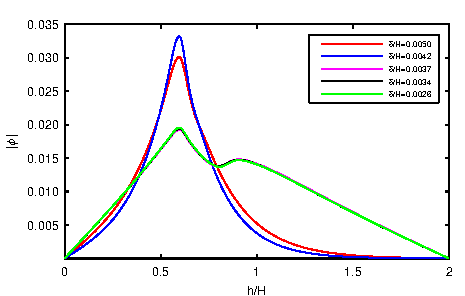
\includegraphics[]{Asymptotic_eig_set3.pdf}
\caption{plot of $|\phi|$ for different shear layer thickness in limit of small shear layer thickness}
\label{Asymptotic_mode}
\end{figure}
\begin{figure}[htb]
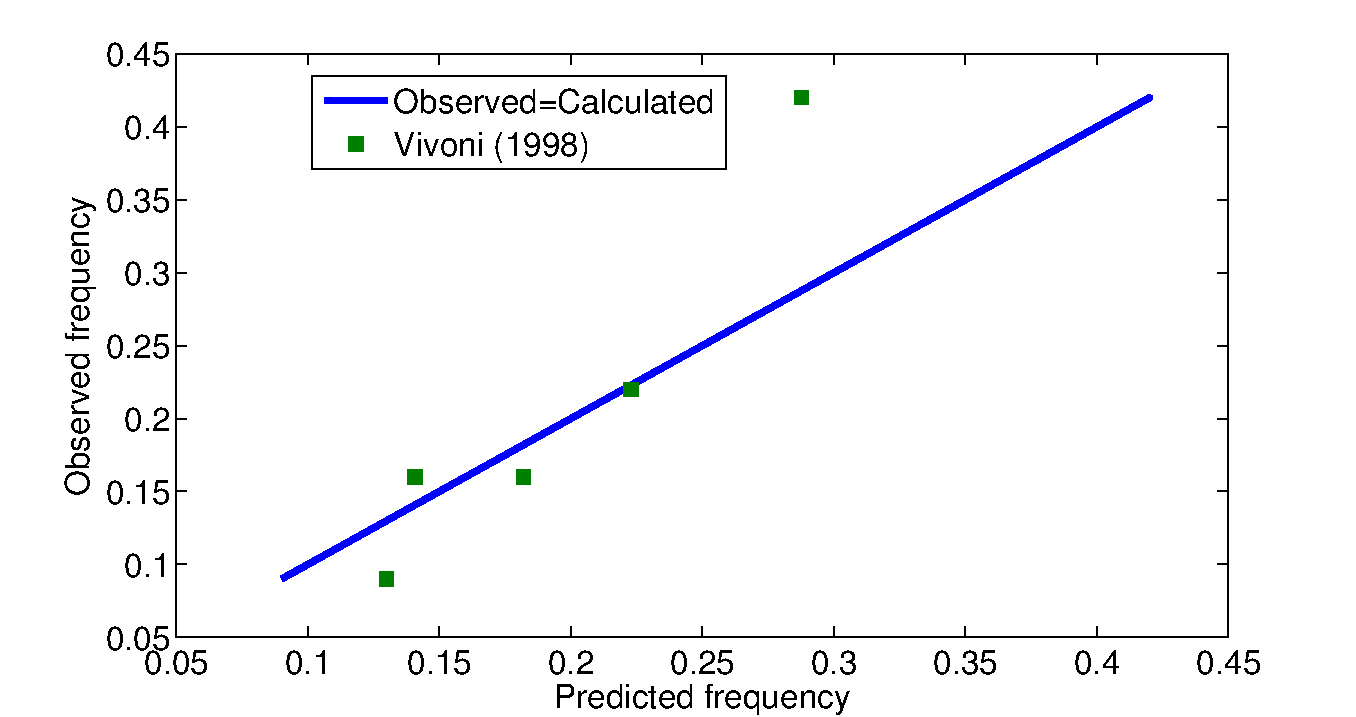
\includegraphics[scale=0.34]{Observed_vs_calculated}
\caption{Comparison between experimently oberved frequency and predicted frequency}
\label{Observed_calculated}
\end{figure}
\newline
Comparison of frequency associated with mode of highest growth predicted by model with that of experimental observations of frequencies in the lab scale experiments is shown in
Figure \ref{Observed_calculated}.
The observed frequencies in the lab scale are associated with the peaks in velocity spectra, frequency of monami and frequency of vortex passage. The agreement between the observed
frequency and the predicted frequency along with shear layer width suggest that monami is associated with the instability of flow comprising shear layer flow and flow above the canopy.
The deviation of predicted frequency from the observed one can be attributed to the various simplification we have made in our model. For real canopy the drag coefficients are known to
decrease from bottom to tip of the grass blades. The turbulent viscosity is also known to vary between the flow of unvegetated region and flow through the canopy. Although these variation
are not central to the mechanism leading to the instability of flow, we believe an improved analysis of flow with these variation in the model might lead to a better agreement between the
observed frequency and the predicted frequency.   
\newline
Numerical investigation of flow in presence of canopy reveal three distinct zone of flow instability which might lead to monami. The occurrence of these three flow instability in a canopy
depends on its submergence ratio and shear layer thickness. Our analysis shows that flow in presence of grass become unstable not only through the mechanism similar to Kelvin-Helmholtz
instability but also through shear instability of flow above the grass for small shear layer thickness and shear instability of flow comprising flow in shear layer with flow above the grass.
Our analysis further predict a threshold criteria characterized by a Reynolds number above which flow become unstable. The predicted value of threshold Reynolds number is $O(100)$, which is 
close to the the Reynolds number corresponding to the observed value of threshold flow speed in the observation of Grizzle. Inclusion of variation of drag coefficient along the grass filament
might lead to better agreement between the observed and predicted frequency of monami. 
%\cite{Delangre06}\cite{Delangre04}\cite{Raupach96}\cite{Nepf99}
%\cite{Nepf02}\cite{Nepf04}\cite{Nepf08}\cite{Nepf08_2}\cite{Raupach11}\cite{Raupach94}
%\cite{Delangre06}
%\begin{figure}[htb]Q
%\subfigure{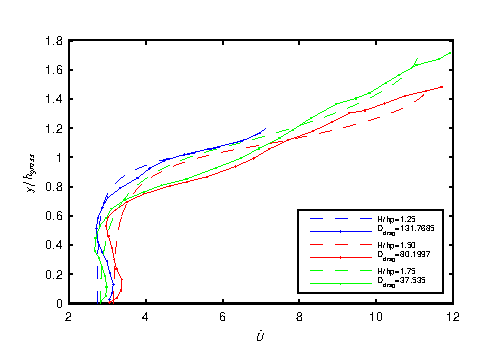
\includegraphics[]{Vivoni_Fig3_6_zero_shear_match}}
%\subfigure{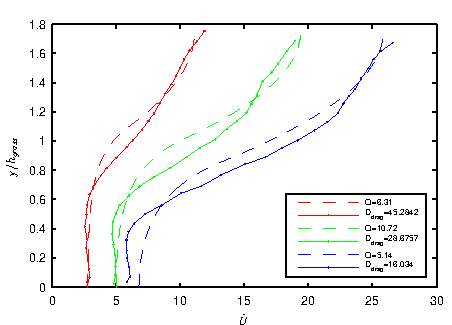
\includegraphics[]{Vivoni_Fig3_7_zero_shear_match}}
%\caption{Comparison between observed and calculated velocity profile}
%\end{figure}
%\begin{figure}[htb]
%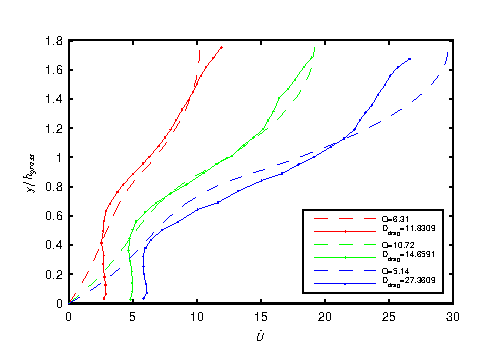
\includegraphics[]{Vivoni_Fig3_7_hb_14match}
%\caption{Comparison between observed and calculated velocity profile,hb=14}
%\end{figure}
%\begin{figure}[htb]
%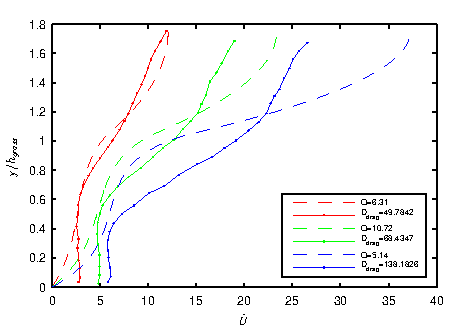
\includegraphics[]{Vivoni_Fig3_7_hb_17match}
%\caption{Comparison between observed and calculated velocity profile,hb=17}
%\end{figure}
\bibliography{Grass}{}
\bibliographystyle{plain}
%\nocite{*}
\end{document}
